\section{When the victim is overconfident: a stress test on GTSRB}
\label{sec:gtsrb}

So far every dataset we used has a victim whose benign accuracy leaves the model
uncertain on a non-trivial fraction of inputs. GTSRB is different: its 43
traffic-sign classes are visually tight, and a ResNet-18 reaches clean
$\ba\!\approx\!100\%$. This makes GTSRB an extreme \emph{high-confidence}
regime rather than just a fourth dataset. We use it as a stress test, asking a
question the per-dataset tables cannot answer: \emph{when the victim is nearly
certain about every clean input, how do the three trigger paradigms---fixed,
flat-spectrum, and optimized-adaptive---each fare?} We poison $1\%$ (189
clean-label samples) of the target class.

% GTSRB stress-test: three trigger paradigms vs an overconfident victim (BA~100).
% Sources: docs/GTSRB-BASELINES.md (baselines), data_faat_summary.csv (FAAT L2=3.5),
%          gtsrb_kst_e48_forget/output_1.log (KST final), KST SSIM at eps20 (clean-label_summary).
\begin{table}[t]
\centering
\small
\setlength{\tabcolsep}{4pt}
\begin{tabular}{l l c c c c}
\toprule
Paradigm & Method & ASR$\uparrow$ & SSIM$\uparrow$ & AC$\downarrow$ & BA \\
\midrule
fixed (visible)   & BadNets-C / MultiBpp & 0.0 & --- & --- & 99.9 \\
fixed (blend)     & Blended-C            & 34.1 & --- & --- & 99.9 \\
flat-spectrum     & KST ($\varepsilon$20) & 0.0 & \textbf{0.94} & --- & 100.0 \\
optimized adaptive& \textbf{FAAT} (Ours) & \textbf{82.7} & 0.72 & 0.76 & 99.8 \\
\bottomrule
\end{tabular}
\caption{\textbf{GTSRB stress test} (43 classes, victim BA$\approx\!100\%$,
$1\%$ clean-label, 189 samples). Fixed triggers are drowned out; the
flat-spectrum KST stays stealthy but cannot flip the overconfident victim
(ASR $0.0$\%); only the optimized adaptive FAAT succeeds, at the cost of
stealth. No method is simultaneously strong and stealthy in this regime.}
\label{tab:gtsrb}
\end{table}


\paragraph{Phenomenon.} Table~\ref{tab:gtsrb} reports the three-way comparison.
Fixed triggers collapse: BadNets-C and MultiBpp reach $\asr\!=\!0$ and Blended-C
only $34.1$. The flat-spectrum \kst{} also fails ($\asr\!=\!0.0$ at the stealthy
$\varepsilon\!=\!20$, SSIM $0.94$). Only the optimized-adaptive \faat{}
succeeds, reaching $\asr\!=\!82.7$ where every fixed baseline is at or near zero.

\begin{figure}[t]
\centering
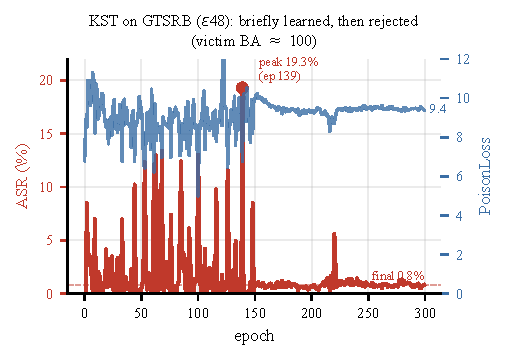
\includegraphics[width=0.92\linewidth]{floats/figures/f12_gtsrb_dynamics.pdf}
\caption{\textbf{KST on GTSRB: briefly learned, then rejected.} ASR peaks at
$19.3\%$ (epoch 139) and collapses to $0.8\%$, while PoisonLoss stays high
($\approx\!9.4$). The overconfident victim (BA$\!=\!100$) resists the
flat-spectrum trigger. Source: \texttt{results/kst\_sdt/gtsrb\_kst\_e48\_forget}.}
\label{fig:gtsrb-dyn}
\end{figure}


\paragraph{Mechanism, with training-dynamics evidence.}
The baselines fail because the clean task is so easy that the model need not
learn any trigger--class association to fit the data; the small fixed signal is
simply drowned out. \kst's failure is more subtle: Figure~\ref{fig:gtsrb-dyn}
shows the victim \emph{briefly learns} the trigger---ASR peaks at $19.3\%$
around epoch 139---then \emph{rejects} it, collapsing to $0.8\%$ while
PoisonLoss stays high ($\approx\!9.4$). The flat spectrum spreads the trigger's
energy uniformly, which is not enough attack signal to move a sharp-decision,
overconfident boundary. This is a property of the regime, not of the method:
the \emph{same} \kst{} at $\varepsilon\!=\!48$ reaches $93.9\%$ on CIFAR-100
(BA $78\%$) and $98.5\%$ on Tiny-ImageNet (BA $55\%$). \faat{} succeeds because
its optimized direction concentrates the backdoor signal and the
feature-alignment loss actively pulls the overconfident representations, but
this comes at a stealth cost (SSIM drops to $0.72$, AC rises to $0.76$, i.e.\
detectable).

\paragraph{Insight: a Pareto swap, and a tightening window.}
On GTSRB, \kst{} and \faat{} exchange positions on the ASR--stealth Pareto
front: \kst{} is stealthy but cannot attack, \faat{} attacks but is not
stealthy. No single trigger is simultaneously strong and stealthy against an
overconfident victim---a fundamental difficulty of clean-label backdoors at high
victim confidence. Along a \emph{confidence axis} (Suppl.),
as victim BA rises (Tiny $55 \to$ CIFAR-100 $78 \to$ CIFAR-10 $95 \to$ GTSRB
$100$), the achievable ASR-and-stealth window narrows and pinches at
BA$\approx\!100$. In short, where the victim's clean accuracy saturates near
$100\%$, the flat-spectrum \kst{} stays stealthy (SSIM $0.94$) but fails to flip
($\asr\!=\!0.8$), while the optimized \faat{} succeeds ($82.7$) at the cost of
stealth (SSIM $0.72$)---an ASR--stealth trade-off that tightens as victim
confidence grows.
